\section{CONTOUR Contour Plot Function}

\subsection{Usage}

This command generates contour plots.  There are several syntaxes for
the command.  The simplest is
\begin{verbatim}
  contour(Z)
\end{verbatim}
which generates a contour plot of the data in matrix \verb|Z|, and will
automatically select the contour levels.  The \verb|x,y| coordinates of the
contour default to \verb|1:n| and \verb|1:m|, where \verb|n| is the number of
columns and \verb|m| is the number of rows in the \verb|Z| matrix.  Alternately,
you can specify a scalar \verb|n|
\begin{verbatim}
  contour(Z,n)
\end{verbatim}
which indicates that you want \verb|n| contour levels.  For more control,
you can provide a vector \verb|v| containing the levels to contour.  If you
want to generate a contour for a particular level, you must pass a
vector \verb|[t,t]| where \verb|t| is the level you want to contour.  If you
have data that lies on a particular \verb|X,Y| grid, you can pass either
vectors \verb|x,y| or matrices \verb|X,Y| to the contour function via
\begin{verbatim}
  contour(X,Y,Z)
  contour(X,Y,Z,n)
  contour(X,Y,Z,v)
\end{verbatim}
Each form of \verb|contour| can optionally take a line spec to indicate the
color and linestyle of the contours to draw:
\begin{verbatim}
  contour(...,linespec)
\end{verbatim}
or any of the other forms of \verb|contour|.  Furthermore, you can supply an
axis to target the \verb|contour| plot to (so that it does not get added to
the current axis, which is the default):
\begin{verbatim}
  contour(axis_handle,...)
\end{verbatim}
Finally, the \verb|contour| command returns a handle to the newly returned
contour plot. 
\begin{verbatim}
  handle = contour(...)
\end{verbatim}
To place labels on the contour plot, use the \verb|clabel| function.
\subsection{Example}

Here is a simple example of a contour plot with the default \verb|x,y|
coordinates:
\begin{verbatim}
--> [x,y] = meshgrid(linspace(-1,1,25),linspace(-2,2,30));
--> z = x.*exp(-x.^2-y.^2);
--> contour(z)
\end{verbatim}
which results in the following plot


\centerline{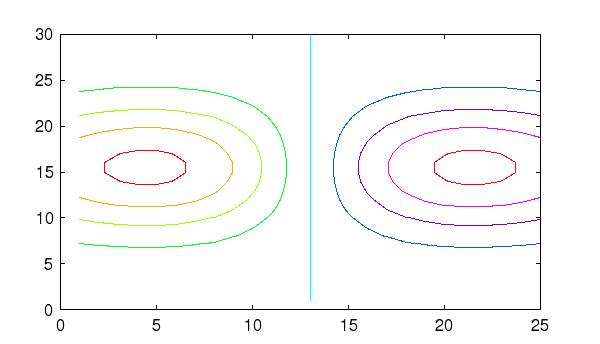
\includegraphics[width=8cm]{contour1}}

Here, we specify the \verb|x| and \verb|y| coordinates explictly
\begin{verbatim}
--> contour(x,y,z)
\end{verbatim}
note that the axis limits have changed appropriately


\centerline{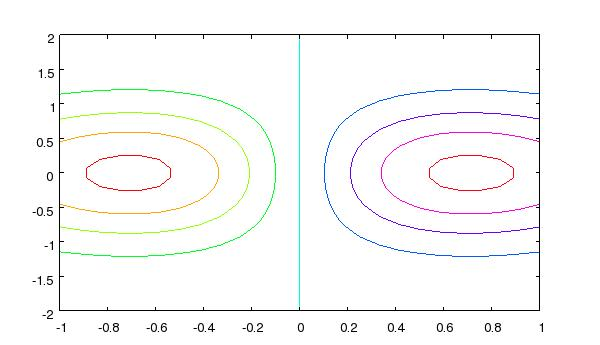
\includegraphics[width=8cm]{contour2}}

By default, contours are created at values selected by FreeMat.  To
provide our own set of contour values (asymmetrically about zero in this
case), we supply them as
\begin{verbatim}
--> contour(x,y,z,[-.4,0.,3])
\end{verbatim}
which is here


\centerline{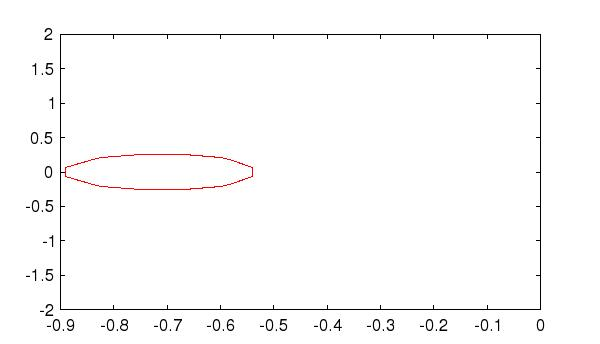
\includegraphics[width=8cm]{contour3}}

Also be default, \verb|contour| uses the current color map and \verb|clim|
limits to determine the coloring of the contours.  Here, we override the
color spec so that we have all black contour
\begin{verbatim}
--> contour(x,y,z,'b-')
\end{verbatim}
which is here


\centerline{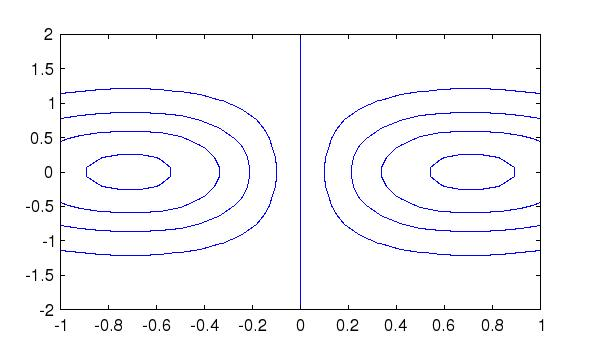
\includegraphics[width=8cm]{contour4}}

